\clearpage
\section{Hardware measurement processing}
\label{supp:note6}

\subsection*{Rice RENEW acquisition, frequency conventions and calibration}
The RENEW analysis uses the registered Rice distributed multi-user MIMO collection.
Each listed file contains 2,001 frame slots, six time-orthogonal client pilot slots,
64 stored receive-stream slots and a noise slot. The selected distributed chain-A
recordings are \texttt{trace-uplink-2022-11-14-2-42-48\_1\_64x6\_0\_63\_chA.hdf5}
(HUB) and \texttt{trace-uplink-2022-11-14-7-10-53\_1\_64x6\_0\_63\_chA.hdf5}
(LO). The carrier is 3.6 GHz and the sample rate is 5 MHz, giving 78.125 kHz
spacing for a 64-point FFT. We retain the recorded ADC scale. Diagonal noise
normalization supplies the receiver's noise metric in these units.

Let $x_{fuan}$ denote the complex ADC sample at time $n$, frame $f$, user $u$
and receive stream $a$. Interleaved signed integers are converted by
$x=(I+\mathrm{i}Q)/32768$. The recorded time-domain pilot and frequency-domain
pilot determine whether the frequency array has been FFT-shifted. For signed
frequency $q\in\{-32,\ldots,31\}$ the two zero-based storage conventions are
\begin{equation}
 b_{\rm centred}(q)=q+32,\qquad b_{\rm native}(q)=q\bmod64.
\end{equation}
Sorting the 48 data tones by signed frequency and taking positions 12, 24 and
36 selects $q=(-13,1,14)$. These map to $(19,33,46)$ in the distributed files
and $(51,1,14)$ in the unshifted colocated LoS files. The four control-pilot
tones and DC are excluded. The decoder explicitly checks the recorded pilot
against both FFT conventions before selecting tones.

The nominal FFT windows are $[176,240)$ and $[256,320)$ within each
1,120-complex-sample slot, with prefix 160 and cyclic prefix 16.
For repetition $r\in\{0,1\}$, with $t_r=176+80r$, the channel estimate is
\begin{equation}
 \widehat h^{(r)}_{fua}(q)=\frac{1}{P(q)}
 \sum_{n=0}^{63}x_{fua,t_r+\ell_u+n}e^{-2\pi\mathrm{i}qn/64},
 \label{supp:eq_renew_fft}
\end{equation}
where $P(q)$ is the recorded pilot and $\ell_u$ is the frozen per-user timing
correction. Calibration scans even shifts from $-64$ to $64$, maximizing
the median log occupied-to-null FFT-energy ratio over reserved frames and
streams, using repetitions indexed 1 through 8. Equal scores prefer the
smallest absolute shift. HUB shifts are $(0,-6,-6,-8,-4,-2)$ samples and LO
shifts are $(-12,-10,-10,-16,-10,64)$. The same shift applies to both windows,
which remain disjoint. The LO sixth-user shift reaches the search boundary,
an observable limitation of this alignment rule.

Frames 0--127 form a reserved calibration prefix. Quality checks use frames
$32,40,\ldots,120$ whose minimum six-user aggregate pilot/noise power ratio
exceeds two. Synchronization uses the first four surviving frames. A receive
stream is retained when at least one user has pilot/noise power at least
6 dB and mean normalized adjacent-LTS coherence at least 0.60, computed
from repetitions 2 through 7 in those calibration frames. This selects
64 HUB and 63 LO streams. The per-stream, per-tone variance is frozen as
\begin{equation}
 \widehat\sigma_a^2(q)=\frac{1}{256}\sum_{f=0}^{127}\sum_{r=0}^{1}
 \left|\mathcal F_{64}\{x^{\rm noise}_{fa,t_r:t_r+64}\}(q)\right|^2,
 \qquad h^{(r)}_{fua}(q)=\widehat h^{(r)}_{fua}(q)/\widehat\sigma_a(q).
\end{equation}
The noise windows use nominal offsets. This is diagonal variance calibration
and carries neither an estimate of cross-stream noise covariance nor a
calibration of radiated transmit power.

\clearpage
\subsection*{RENEW replay, exclusions and mirrored-directory evidence}
For each post-prefix frame, all six pilots must be present, all retained
streams must contain nonzero pilot samples and the extracted noise powers
must be positive. Each user's median retained-stream decision-window to
preceding-guard power ratio must be at least two. Every failed frame remains
in the denominator of 1,873. The early LTS determines the schedule, powers,
filters and recorded-input interval. The identical action is evaluated on
the later LTS as a reference proxy. Its median difference from the early
lower endpoint is $-2.501$ (HUB) and $-4.873$ (LO) bit/s/Hz. All retained
later references fall below that endpoint. This discrepancy limits temporal
interpretation of the early-input certificate.

\begin{table}[htbp]
\centering\small
\caption{RENEW full-capture and nested-window results. A useful decision has
$G\leq0.10$ bit/s/Hz and elapsed time $\leq250$ ms. Nested entries list
$K=2,4,6$ in that order and give medians over 32 accepted windows per listed
stratum. Source-directory labels are preserved.}
\label{supp:table8}
\begin{tabular}{lrrrrr}
\hline
Full chain-A capture & RF & Retained/1,873 & Useful/1,873 & Median $G$ & Median ms\\
\hline
Distributed HUB LoS &64&1,870&1,867&0.00005190&2.7548\\
Distributed LO LoS &63&1,769&1,037&0.07479139&2.7082\\
\hline
\multicolumn{6}{l}{Nested sensitivity, 32 windows per $K$}\\
Directory and chain & RF & \multicolumn{3}{c}{Median $G$ for $K=2,4,6$} & Useful\\
\hline
Colocated HUB LoS A &63&0.0003919&0.00004754&0.00004195&32/32 each\\
Colocated HUB LoS B &63&0.0005810&0.00004160&0.00374474&32/32 each\\
Colocated HUB NLoS A &64&0.0003452&0.00007622&0.00006767&32/32 each\\
Colocated HUB NLoS B &64&0.0005105&0.00004837&0.00007956&32/32 each\\
Distributed HUB LoS A &64&0.0003452&0.00007622&0.00006767&32/32 each\\
Distributed HUB LoS B &64&0.0005105&0.00004837&0.00007956&32/32 each\\
Distributed LO LoS A &63&0.0015542&0.00016973&0.00012370&32/32 each\\
\hline
\end{tabular}
\end{table}
\subsection*{Chronological directional calibration and exhaustive pairing}
The first 128 frames continue to determine timing, RF selection and noise variance only. Among the eligible post-prefix frames, the first 256 form a new chronological calibration set and the remainder form a disjoint test set. The scheduling map takes only the early pilot. For frame $f$, let $\Delta h_{fus}=h^{(1)}_{fus}-h^{(0)}_{fus}$ and let $\bar v_{fis}$ be the unit-normalized early-input filter. We use scalar whole-frame scores
\[
 s_{F,f}=\max_{u,s}\|\Delta h_{fus}\|_2,\qquad
 s_{P,f}=\max_{(i,j,s)\text{ scheduled}}\max_{k\in\{i,j\}}
 |\bar v_{fis}^{H}\Delta h_{fks}|.
\]
Both receiver directions in each pair are included. The 251st sorted score of 256 calibration frames, rounded outward, supplies each radius. The same projected radius is used for every desired/interference projection within a frame. Vector and projected events each receive error budget 0.025. The test has 1,614 HUB and 1,513 LO frames. Every lower and upper certificate is replayed by the separate numerical checker. Empirical floor coverage counts $R_{\rm later}\geq L_P$; interval coverage uses $\max(L_P,L_F)\leq R_{\rm later}\leq U_F$. The reported projected width is $U_F-L_P$.

These residuals include pilot noise, synchronization differences and channel evolution. No component is identified separately. The temporal split avoids reusing calibration residuals for testing, but successive frames are not independent replicates. We therefore do not use the conformal rank formula as evidence of population coverage, or attach an independent-binomial confidence interval to these recording-level fractions. All coverage statements concern the second observable LTS and the stored early-input action.

At six users and three labelled tones, sorting the two user indices within each pair leaves $6!/2^3=90$ schedules. We enumerate all 90 with fixed powers of 0.10 and the MMSE pair rate on the early input. This is exhaustive over the stated discrete set; the rates are floating-point numerical evaluations. Its optimum is a feasible reference for the continuous-power model, not that model's exact optimum.


\subsection*{Phase-invariant scores and the thermal-noise benchmark}
For each user and frame we calculate the phase of the inner product of the early and later channel vectors concatenated over all retained streams and three tones. Over test user--frame pairs, median absolute rotations are 0.041899 rad on HUB (IQR 0.019987--0.071188) and 0.259930 rad on LO (0.233082--0.286302). Dividing by \(2\pi(16~\mu{\rm s})\) gives equivalent absolute frequency offsets of 0.416773 kHz (0.198816--0.708123) and 2.585568 kHz (2.318505--2.847896). These conversions attribute the entire phase change to frequency offset for scale; the replay does not identify a causal oscillator model.

For the projected magnitude score and phase-aligned vector score, respectively, we use
\[
s^{\rm mag}_{P,f}=\max_{(i,j,s),\,k\in\{i,j\}}
\left||\bar v_{fis}^Hh^{(1)}_{fks}|-|\bar v_{fis}^Hh^{(0)}_{fks}|\right|,
\qquad
s^{\rm ph}_{F,f}=\max_{u,s}\min_\theta
\|e^{-{\rm i}\theta}h^{(1)}_{fus}-h^{(0)}_{fus}\|_2 .
\]
The vector alignment minimizes separately for each user/tone; the diagnostic phase above is instead one concatenated phase per user/frame. Both scores retain the original 256 calibration frames, rank 251 and test frames. If a magnitude residual is at most \(b_{ik}\), the desired amplitude is bounded below by \((|\bar v_i^Hh_i^{(0)}|-b_{ii})_+\), and the interfering amplitude above by \(|\bar v_i^Hh_j^{(0)}|+b_{ij}\). The SINR is increasing in the first squared amplitude and decreasing in the second, proving the projected floor conditionally on those bounds; the vector oracle is unchanged by user/tone phase rotations. The implementation checks rate/score phase invariance and replays every numerical certificate.

As a thermal-noise-only benchmark, independently drawn proper complex pilot errors of unit variance give difference variance two. A unit-filter projection then has tail probability \(\exp(-x^2/2)\); a union bound over 12 projections gives the 97.5\% threshold \(\sqrt{2\log(12/0.025)}=3.51391\). The expected maximum for 12 independent projections is 2.44453. Holding the observed early filters fixed and retaining correlations between projections, 16,384 Monte Carlo blocks per capture give expected maxima 2.44987 (HUB) and 2.44705 (LO), with Monte Carlo standard errors 0.00377 and 0.00378. This benchmark isolates noise and does not model the dependence of estimated filters on their noisy pilots, cross-stream noise correlation, or drift. The observed raw radii of 87.36 and 165.26 greatly exceed it. Removing phase sensitivity raises the floors, yet LO joint-event coverage remains 75.74\%, below nominal 95\%; its universal floor coverage is sustained by slack.

\begin{table}[htbp]\centering\small
\setlength{\tabcolsep}{4pt}
\caption{Chronological RENEW calibration against the observable second LTS. The first 256 eligible post-prefix frames calibrate the radii; all remaining eligible frames test the frozen rule. Rates and widths are bit/s/Hz; radii are in whitened digital channel units. Coverage fractions describe these temporally dependent recordings, without binomial population confidence intervals. The equal-power reference exhausts all 90 labelled pairings at 0.10 per user, with optimal linear combining, on every eligible early input. It is not the continuous-power optimum.}\label{supp:hardware_calibration}
\begin{tabular}{lll}\toprule
Quantity & HUB & LO\\
\midrule
Calibration frames & 256 & 256\\
Test frames & 1614 & 1513\\
Vector radius & 100.7147 & 189.2814\\
Projected radius & 87.3634 & 165.2563\\
Later rate above projected floor (\%) & 100.00 & 100.00\\
Later rate in combined interval (\%) & 100.00 & 100.00\\
Both residual events hold (\%) & 97.40 & 70.26\\
Median projected lower rate & 3.754 & 1.292\\
Median vector upper rate & 26.831 & 28.118\\
Median projected interval width & 23.075 & 26.830\\
Positive projected floors & 1614 & 1513\\
Median early ceiling minus equal-power optimum & 3.3257e-05 & 6.8581e-05\\
\bottomrule\end{tabular}
\end{table}
The projected interval is $[L_P,U_F]$; the combined lower endpoint for the interval-coverage diagnostic is $\max(L_P,L_F)$. The early ceiling minus the enumerated equal-power optimum is reported separately from the achieved-action gap. The exhaustive comparison includes both calibration and test frames; calibrated coverage uses test frames only. The 70.26\% joint residual-event coverage on LO does not support a nominal 95\% calibration claim, even though the conservative rate floors cover all observed test rates.



The sensitivity replay selects 32 integer-spaced frames from 128 to 1,999,
with users $1{:}K$ and tone sets $\{1\}$, $\{-13,14\}$ and $\{-13,1,14\}$
for $K=2,4,6$. Thus the user subsets are nested and each replay has $K/2$
tones. Its calibration uses candidate prefix frames $(32,56,80,104)$,
retaining the pilot-present subset for noise estimation and quality masking.
These smaller-prefix estimates explain why its gaps differ from the
full-capture replay. LO chain B failed calibration and contributes no window.

\begin{figure}[htbp]
\centering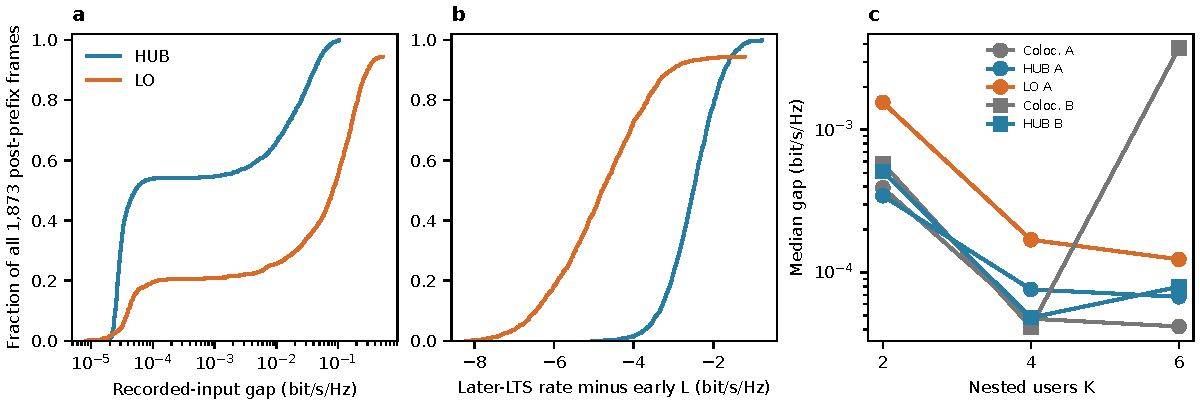
\includegraphics[width=\linewidth]{supplementary/figures/sfig7.pdf}
\caption{RENEW recorded-input gap distributions (a), later-LTS fixed-action
rate minus early lower endpoint (b), and nested-window sensitivity (c).
Both ECDFs use all 1,873 post-prefix frames per mode as their denominator,
so their final heights expose abstentions. Panel c omits the mirrored NLoS
directory curves, which coincide with the distributed HUB curves.}
\label{supp:fig7}
\end{figure}

\clearpage
\subsection*{Provenance and acquisition scope}
The colocated HUB NLoS and distributed HUB LoS directory entries have matching
filenames, lengths and acquisition timestamps. Independently requested common
byte ranges have matching SHA-256 digests for 24/24 chain-A ranges and 22/22
chain-B ranges. Sampled pilot and noise arrays also match. The evidence
supports probable directory mirroring. Physical placement remains dependent
on source-side provenance. These entries therefore add no independent
replication. Full-capture SHA-256 digests are
\begin{quote}\footnotesize\ttfamily
HUB\quad\nolinkurl{aec556198de39208757fddc294af77d4f701d7a24b9f1feb3f1fdc09d36bc0d2}\\
LO\quad\nolinkurl{e5fabc009dce96e527b6919ce744f0b41408f337e0d5334b8dadfa0f13699844}.
\end{quote}
Each distributed clock mode supplies one acquisition. Frames, user subsets,
RF chains and tones are repeated observations within this evidence base.
The six-user offline scheduling counterfactual has no measured counterfactual
payload throughput. The two disjoint LTS windows provide a temporal proxy
comparison with an empirically substantial discrepancy. Hardware population
coverage and a causal clock-mode comparison require additional acquisitions.

The separate CPU implementation reconstructed the full RENEW distributions from archived accepted-frame
and abstention records. Its authenticated source spot check fetched frame 128
and calibration-noise frames $(56,80,104)$ for HUB and $(80,104)$ for LO,
verifying respectively 18 and 14 source pages. Recomputed mean pair overlaps
were 0.08521393847151353 and 0.06809478943705848, agreeing with archived values
to floating-point precision. Complete distributed IQ captures were unavailable
to that audit. The present supplement regenerates the full distributions from
those archived derived rows and verifies their counts.

\subsection*{Rice Argos six-user correlation statistic and quality masks}
The three Argos UHF recordings are the 28 November 2015 static (14:39:47),
environmental-mobility (14:43:08) and mobile (14:47:06) acquisitions. They contain
12,017, 12,014 and 12,018 frames respectively, six user slots and a seventh
noise slot, recorded through eight RF streams. The analysis protocol reserves
frames 0--63 for RF qualification and fixes 32 interior evaluation frames as
\begin{equation}
 f_j=64+\left\lfloor\frac{(2j+1)(n_f-64)}{64}\right\rfloor,
 \qquad j=0,\ldots,31.
\end{equation}
Each RF record reshapes into seven slots of 224 complex samples. The two
64-sample LTS windows start at zero-based offsets 47 and 111. After a centred
FFT, occupied bins are $6{:}31$ and $33{:}58$, equivalently signed tones
$-26{:}-1$ and $1{:}26$. The remaining 12 bins contain DC and guard tones.
The seventh slot is excluded from user-pair statistics.

Let $H^{(r)}_{fua}(q)$ be the resulting occupied-bin vector. The quality
measure divides mean occupied-bin energy by mean null-bin energy, averaging
both LTS windows. Adjacent-LTS coherence is the magnitude of their tonewise
inner product divided by the product of their norms. An RF stream is
qualified if at least one user has median calibration concentration at least
6 dB and median coherence at least 0.60. All eight streams qualify in every
recording. An evaluation frame must supply all six finite, nonzero channel
vectors on all 52 tones, at least two qualified streams, and for every user
median concentration at least 3 dB and median coherence at least 0.50 over
retained streams. Failed frames are retained as abstentions and never replaced.

\clearpage
For unordered pair $(u,v)$, define
\begin{equation}
 \rho^{(r)}_{fuv}(q)=
 \frac{|(H^{(r)}_{fu}(q))^{\!H}H^{(r)}_{fv}(q)|^2}
 {\|H^{(r)}_{fu}(q)\|^2\|H^{(r)}_{fv}(q)\|^2},\quad
 c^{(r)}_{fuv}=\frac1{52}\sum_q\rho^{(r)}_{fuv}(q),\quad
 \bar c^{(r)}_f=\frac1{15}\sum_{u<v}c^{(r)}_{fuv}.
\end{equation}
Supplementary Table~\ref{supp:table9} gives medians and quartiles of $\bar c^{(r)}_f$ over
qualified frames, with paired changes calculated before taking the median.
Supplementary Fig.~\ref{supp:fig8} instead gives the median of each pair's
$c^{(r)}_{fuv}$ over those same frames. Their different aggregation orders
are explicit. The heatmaps are recomputed from locally retained IQ windows,
with all 99 source-range digests and three frame-zero digests checked. Every
recomputed pair/frame mean agrees with the archived scalar statistic to
absolute tolerance $2\times10^{-13}$ plus relative tolerance $10^{-12}$.
Controls cover orthogonal, identical, zero and phase-rescaled vectors.

\begin{table}[htbp]
\centering\small
\caption{Argos first- and second-LTS spatial correlations. Brackets are
within-recording first and third quartiles. The unfiltered column includes
all 32 finite planned frames. All values are dimensionless.}
\label{supp:table9}
\begin{tabular}{lrrrrr}
\hline
Recording & Retained & First LTS & Second LTS & Paired change & Unfiltered first\\
\hline
Static &31/32&0.2250&0.2378&0.0176&0.2224\\
 & &[0.2051,0.2405]&[0.2230,0.2498]&[-0.0036,0.0305]&\\
Environmental &32/32&0.2402&0.2533&0.0083&0.2402\\
 & &[0.2250,0.2533]&[0.2387,0.2614]&[0.0003,0.0215]&\\
Mobile &22/32&0.2250&0.2430&0.0108&0.2288\\
 & &[0.2158,0.2356]&[0.2302,0.2514]&[0.0033,0.0304]&\\
\hline
\end{tabular}
\end{table}
\begin{figure}[htbp]
\centering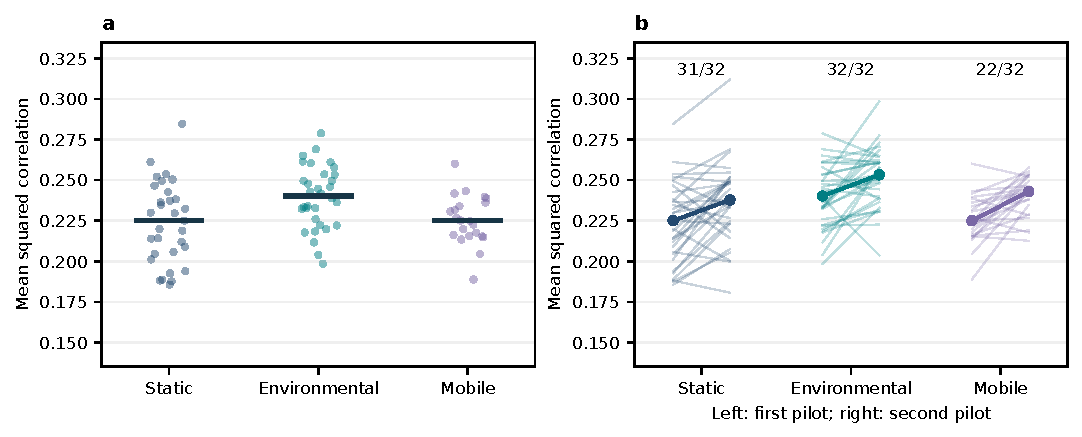
\includegraphics[width=0.92\linewidth]{supplementary/figures/sfig8.pdf}
\caption{Argos spatial overlap on two recorded pilots. \textbf{a}, First-LTS mean squared correlation on each qualified frame, with horizontal segments marking medians. \textbf{b}, Thin lines join the first and second LTS from the same frame; thick lines join the medians. Counts give qualified frames out of 32 planned frames. Both repetitions use identical RF masks. These panels describe spatial separation, not paired-payload throughput.}
\label{supp:fig8}
\end{figure}
The three recordings describe one array setup with one recording per
condition. Their spatial correlations support a small-load hardware
description. Supplementary data contain derived scalar summaries and hashes.
Access to the original IQ and reconstructed complex channels follows Rice's research-use terms.


Platform credit belongs to the Rice RENEW team and M. Zafari's distributed
multi-user MIMO dataset (doi:10.21227/74ez-b275), and to C. Shepard,
J. Ding, R. E. Guerra and L. Zhong, \emph{Understanding Real Many-Antenna
MU-MIMO Channels} (Asilomar 2016), for the Argos recordings.
